% ============================================================= %
%  --- Bell Database Article ---
% ============================================================= %

\documentclass[11pt, a4paper]{article}

% ------------------------------------------------------------- 
% Packages
% -------------------------------------------------------------
\usepackage{microtype} % Better typography
\usepackage{fontspec} % For loading fonts
\usepackage{fontawesome5} % For icons
\usepackage{parskip} % No paragraph indentation
\usepackage{ragged2e} % For better justification control
\usepackage{hyphenat} % For hyphenation control
\usepackage[left=2cm,right=2cm,top=2cm,bottom=2cm]{geometry} % Page margins
\usepackage{pgfplots} % For plots
\usepackage{pgf-pie} % For pie charts
\usepackage{amsmath} % For math
\usepackage{caption} % For captions
\usepackage{hyperref} % For hyperlinks

\usepackage{natbib}  % Advanced citation commands
\usepackage{url}     % For formatting URLs
\usepackage{doi}     % For DOI hyperlinks

% -------------------------------------------------------------
% Font
% -------------------------------------------------------------
\usepackage{fontspec}
\setmainfont{Fira Code}


% -------------------------------------------------------------
% Styles
% -------------------------------------------------------------
\renewcommand{\abstractname}{} % Remove abstract title
\newlength{\abstractwidth}
\setlength{\abstractwidth}{0.8\textwidth}

% -------------------------------------------------------------
% Codeblocks
% -------------------------------------------------------------
\usepackage{listings} % For codeblocks
\usepackage{xcolor} % For colors
\definecolor{lgray}{gray}{0.9} % Light gray color

\lstdefinelanguage{CSS}{
  keywords={
    color, background, font, margin, padding, border, display, position,
    width, height, top, left, right, bottom, float, clear, overflow,
    text-align, vertical-align, line-height, letter-spacing, word-spacing,
    text-decoration, text-transform, font-family, font-size, font-weight,
    font-style, list-style, list-style-type, list-style-position,
    table-layout, border-collapse, border-spacing, caption-side, empty-cells,
    content, cursor, outline, visibility, z-index, zoom, filter, opacity,
    transition, animation, transform, box-shadow, text-shadow, border-radius,
    background-image, background-repeat, background-position, background-size,
    @media, @keyframes, !important
  },
  keywordstyle=\color{magenta},
  comment=[l]{//},
  morecomment=[s]{/*}{*/},
  commentstyle=\color{green},
  stringstyle=\color{purple},
  sensitive=true,
  morestring=[b]",
  morestring=[b]',
}

\lstdefinestyle{Pythonstyle}{
    language=Python,
    backgroundcolor=\color{lgray},
    commentstyle=\color{green},
    keywordstyle=\color{magenta},
    numberstyle=\tiny\color{gray},
    stringstyle=\color{purple},
    basicstyle=\ttfamily\footnotesize,
    breakatwhitespace=false,
    breaklines=true,
    captionpos=b,
    keepspaces=true,
    numbers=left,
    numbersep=5pt,
    showspaces=false,
    showstringspaces=false,
    showtabs=false,
    tabsize=2
}

\lstdefinestyle{CSSstyle}{
    language=CSS,
    backgroundcolor=\color{lgray},
    commentstyle=\color{green},
    keywordstyle=\color{magenta},
    numberstyle=\tiny\color{gray},
    stringstyle=\color{purple},
    basicstyle=\ttfamily\footnotesize,
    breakatwhitespace=false,
    breaklines=true,
    captionpos=b,
    keepspaces=true,
    numbers=left,
    numbersep=5pt,
    showspaces=false,
    showstringspaces=false,
    showtabs=false,
    tabsize=2
}

\lstdefinestyle{HTMLstyle}{
    language=HTML,
    backgroundcolor=\color{lgray},
    commentstyle=\color{green},
    keywordstyle=\color{magenta},
    numberstyle=\tiny\color{gray},
    stringstyle=\color{purple},
    basicstyle=\ttfamily\footnotesize,
    breakatwhitespace=false,
    breaklines=true,
    captionpos=b,
    keepspaces=true,
    numbers=left,
    numbersep=5pt,
    showspaces=false,
    showstringspaces=false,
    showtabs=false,
    tabsize=2
}


% ============================================================== %
%  --- Document Information ---
% ============================================================== %

\title{\Huge Structuring Bell Heritage: A Comprehensive Database Schema and Framework for Carillons and Bells}
\author{\LARGE{Jakob De Vreese} \\ 
\texttt{\small{jakobdevreese@gmail.com}} \\
\LARGE{Rachel Perfecto} \\
\texttt{\small{perfecto.rachel@gmail.com}}}
\date{March 2025}

% ============================================================== %
%  --- Document ---
% ============================================================== %

\begin{document}

% -------------------------------------------------------------
% Title Page
% -------------------------------------------------------------
\begin{titlepage}
    \newgeometry{top=4cm}
    \maketitle
    \thispagestyle{empty}
    \vspace{1cm}
    \begin{center}
        \small{last updated: \today}
    \end{center}
    \vspace{2cm}
    
    \begin{center}
        \rule{\textwidth}{0.4pt}
        \vspace{1em}
        
        \begin{minipage}{\abstractwidth}
            \setlength{\rightskip}{0pt plus 1fil} % Allow extra stretch on each line
            \justifying
            \noindent
            This research presents a standardized \textbf{database schema} for campanological documentation, developed initially for the \textbf{Ghent Carillon Association} while designed for broader adoption. The work aims to identify the \textbf{minimal structural requirements} for comprehensively documenting bells and carillons within a standardized framework, facilitating cross-institutional data exchange. In addition, a complementary \textbf{open-source Django web application} is being developed to implement this schema, and it will be fully documented and made publicly available for use by all interested organizations in future publications.
          \end{minipage}
        
        \vspace{1em}
        \rule{\textwidth}{0.4pt}
    \end{center}

    \restoregeometry
\end{titlepage}

% -------------------------------------------------------------
% Table of Contents
% -------------------------------------------------------------

\clearpage
\setcounter{page}{1}
\pagenumbering{arabic}
\tableofcontents
\clearpage

% -------------------------------------------------------------
% Begin of the document
% -------------------------------------------------------------
\section{Abstract}

This research addresses an important challenge in campanology: the fragmentation, inconsistent and incompatible documentation of bell heritage data across organisations, institutions and researchers. We propose a standardized database schema that establishes minimal structural requirements for comprehensive bell documentation, developed initially for the \textbf{Ghent Carillon Association} but designed for broader adoption within the international campanological community. Our model identifies four essential entities — \textbf{bells, founders, towers, and carillons} — with their core attributes and relationships, creating a framework that balances standardization with flexibility.

The bell entity forms the central component of our schema, documenting physical properties, historical information, and contextual elements. We give special attention to the founder entity, which presents unique modeling challenges due to its historical complexity — accommodating individual craftsmen, family workshops, and commercial enterprises across centuries with varying naming conventions and organizational structures. Similarly, our tower entity captures not only geographical location but contextual information about the installation environment, while the carillon entity enables documentation of bell collections as functional musical instruments.

This database schema enables independent organizations to maintain autonomous customized databases while ensuring structural compatibility for potential \textbf{cross-institutional data exchange and aggregation}. By identifying minimal required fields and conventions while allowing for extension and customization, our approach accommodates both amateur enthusiasts with limited technical resources and professional researchers with more complex documentation needs. An accompanying open-source Django web application implements this schema, providing organizations with a customizable, self-hostable solution for campanological data management with built-in file attachment capabilities for multimedia documentation. This will be presented in later publications.

By establishing this foundation, we could facilitate the transformation of isolated bell documentation efforts into an \textbf{interconnected network} of compatible datasets, enhancing opportunities for collaborative research and comprehensive analysis across the field of campanology. This standardized framework represents a significant step toward preserving and studying bell heritage through structured, accessible, and interoperable data management. We also propose a set of \textbf{best practices} for data collection and field measurment to further enhance the quality and consistensy of the data.

\section{Introduction}

In the field of campanology, a wealth of valuable data is continuously gathered by both professional researchers and dedicated enthusiasts. This information encompasses a diverse range of attributes: physical dimensions of bells, acoustic properties, historical provenance, inscriptions, decorative elements, mechanical configurations, and the compositional arrangements of bell sets within carillons and towers. Despite this rich accumulation of knowledge, the campanological field faces a significant challenge: the lack of standardized methods for structuring, storing, gathering and sharing this information in a consistent and accessible manner.

The current diverse and wide landscape of campanological data management is characterized by fragmentation and inconsistency. Individual researchers, institutions, and bell enthusiasts typically develop their own valuable documentation methods, resulting in a patchwork of incompatible datasets. These range from handwritten notes and spreadsheets to custom-built databases with idiosyncratic schemas. While these approaches may serve immediate project needs, they create substantial barriers to knowledge sharing, comparative analysis, and comprehensive research across the broader field.

This fragmentation presents several critical limitations:

\begin{itemize}
    \item \textbf{Restricted Accessibility:} \\
        Valuable research remains siloed within individual projects or institutions, limiting potential insights from combined datasets.
    \item \textbf{Duplication of Effort:} \\
        Researchers frequently redocument the same bells due to lack of awareness or access to existing documentation.
    \item \textbf{Inconsistent Terminology:} \\
        The absence of standardized vocabulary and measurement protocols creates difficulties in comparing data between sources.
    \item \textbf{Limited Analytical Capacity:} \\
        The inability to easily aggregate distributed datasets hinders comprehensive statistical analysis and pattern recognition across larger samples.
\end{itemize}

This paper proposes a solution to these challenges through the development of a comprehensive database schema and framework specifically designed for campanological research. Our approach balances the need for standardization with the flexibility required to accommodate the diverse documentation needs across the field.

This research is the first step in a wider project that will culminate in an open-source web application that can be used and customized by indivituals and organizations to document their bell heritage. The wider goal of this project is:

\begin{enumerate}
    \item Design and propose a flexibel, comprehensive and adaptable database schema for campanological data management.
    \item Develop an open-source, easy to use, web application that implements this schema.
    \item Facilitate the integration of distributed campanological datasets, enabling comprehensive analysis and collaborative research.
\end{enumerate}

\subsection{Case Studies}

We see in the field of campanology a lot of different very good efforts in documenting local bell heritage and carillon culture. These efforts are cructial, but the data is often not easily used for other purposes than manually look up local data. Some of these notable efforts are listed below, that are used as inspiration for our work.

\begin{enumerate}
    \item \textbf{Towerbells}: A database of carillons and bells in North-America and elsewhere in the world. \href{https://www.towerbells.org/}{link}
    \item \textbf{Dove's Guide of Church Bell Ringers}: A database of bells in the United Kingdom and towers in the world containing bells hung for English style "full circle" change ringing, but increased to other bells of interest. \href{https://dove.cccbr.org.uk/}{link}
    \item \textbf{Bell Founders Database}: A database of Bell Founders accessible in different ways, maintained by Peter Dyson and Matt Dyson. \href{https://www.bellfounders.net}{link}
    \item \textbf{The Nautical Archaeology Digital Library}: A database of ship bells from the 16th and 17th centuries. \href{https://shiplib.org/index.php/collections/artifact-collections/early-ship-bells-database/}{link} 
    \item \textbf{klokkenwiki.nl}: A Dutch wiki website abouw bells, bellfounders and heritage in the Netherlands. \href{https://www.klokkenwiki.nl}{link}
\end{enumerate}

There are more databases and efforts in the field of campanology, but we did not have time yet to document them all. If you know a database or effort that is not listed here, please let us know.

\subsection{Background}

The Ghent Carillon Association \"Clocke Roeland\" is a non-profit organization dedicated to the preservation and promotion of the carillon and bell heritage of Ghent and the surrounding region. The organization undertakes a range of activities, including researching and documenting bells. To support these efforts, and to address the challenges of fragmented data mangagement, and difficulties to share data, the organization initiated this project.
    
\section{Database Schema}

When designing a database schema for campanological data, we must consider the diverse range of attributes. We start with the smallest unit we want to document: the bell. A bell has a set of physical properties, such absence diamieter, height, weight and inscriptions, but also has a set of relationships with other entities, like bell founder. A bell hangs most of the time in a tower, wich gives away the geographical location, and can be part of a larger entity, the carillon. When we take this into account, we can start designing the database schema.

\begin{figure}[h!]
    \centering
    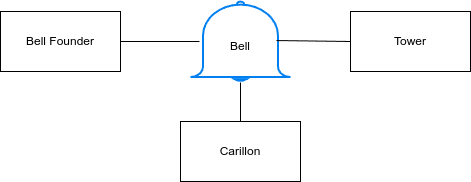
\includegraphics[width=0.8\textwidth]{images/basic_entities.png}
    \caption{Basic entities in the campanological database schema.}
    \label{fig:basic-entities}
\end{figure}

When we look at the basic entities in the campanological database schema, we see that the bell is the central entity. When we put this central in our database, and we add the relationships between the entities, we get a readable and 
connectible database. To lay the basis for a standardization in this field, we off course need more. We want a minimum of fields that every database in our field should have, and a standardized way of taking basic field measurements and naming conventions.

\subsection{Bell}

The bell is our starting point. The minimal attributes needed to describe a bell, in a way that it can't be confused with another bell, are:

\begin{itemize}
    \item \textbf{Founder:} \\
        The founder of a bell, this can be a person or a company. (Other entity)
    \item \textbf{Weight:} \\
        The weight of the bell (in kilograms)
    \item \textbf{Pitch:} \\
        The pitch of the bell (in Hertz)
    \item \textbf{Diameter:} \\
        The diameter of the bell (in centimeters)
    \item \textbf{Height:} \\
        The height of the bell (in centimeters)
    \item \textbf{Inscriptions:} \\
        The inscriptions on the bell in words
    \item \textbf{Year:} \\
        The year the bell was cast.
    \item \textbf{Location:} \\
        The location of the bell. (Other entity)
\end{itemize}

Other attributes can be added to the bell entity, but these are the minimal attributes needed to describe a bell. The researchers should strive to document these attributes as complete as possible for all bells.

\begin{figure}[h!]
    \centering
    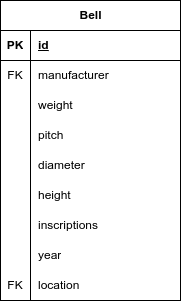
\includegraphics[width=0.3\textwidth]{images/bell.png}
    \caption{Minimal attributes for the bell entity.}
    \label{fig:bell-entity}
\end{figure}

\subsection{Founder}

The Founder entity presents unique modeling challenges in campanological documentation due to its inherent complexity. 
Bell founders may be individuals, family workshops, commercial enterprises, or combinations thereof, with varying historical 
naming conventions and organizational structures spanning centuries. Furthermore, founders often exhibit complex 
relationships — individuals may work under multiple establishments, companies may undergo name changes, and master founders 
may collaborate while maintaining distinct signatures.

To accommodate this complexity while ensuring standardization, and simplicity, we propose a structured approach to founder documentation with the following attributes:

\begin{itemize}
    \item \textbf{Primary Name:} The canonical name used for indexing and primary identification
    \item \textbf{Alternative Names:} Historical variants, orthographic differences, and aliases
    \item \textbf{Company Name:} May be blank or contain the name of a company or workshop.
    \item \textbf{Activity Period:} Documented years of bell-founding activity
    \item \textbf{Geographic Locations:} Principal locations of operation
\end{itemize}

This approach allows for precise documentation of complex cases: a bell signed by individual craftsmen working under a company name can be properly attributed to both entities while maintaining their relationship. Similarly, when a founder worked across multiple establishments during different periods, these associations can be preserved without sacrificing searchability. The schema enables researchers to query by either individual name or establishment, retrieving the complete attribution context 
regardless of entry point.

By implementing this structured yet flexible approach to founder documentation, we establish a foundation that accommodates 
historical complexity while facilitating standardized access and cross-referencing across distributed datasets.

\begin{figure}[h!]
    \centering
    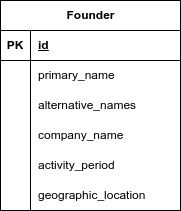
\includegraphics[width=0.3\textwidth]{images/founder.png}
    \caption{Minimal attributes for the founder entity.}
    \label{fig:founder-entity}
\end{figure}

\subsubsection{Relationship Founder - Bell}

The relationship between founders and bells represents a \textbf{many-to-many association} with significant temporal complexity. While a founder typically casts numerous bells throughout their career, a single bell may also be associated with multiple founders across its lifetime. This occurs when bells are recast, restored, or undergo significant modifications that warrant documentation. 

To properly capture this historical complexity, we require a dedicated relationship table that includes temporal attributes documenting when work was performed, the nature of the intervention (casting, recasting, restoration), and whether the relationship represents the bell's original creation or a subsequent modification. This approach allows researchers to trace the complete lifecycle of a bell while maintaining accurate attribution of each craftsman's contribution to its current state. The relationship entity contains attributes such as:

\begin{itemize}
    \item \textbf{Date of Work:} When the founding or modification occurred
    \item \textbf{Type of Intervention:} Original casting, recasting, repair, etc.
    \item \textbf{Primary Attribution:} Whether this represents the bell's original creation
    \item \textbf{Additional Notes:} Documentation of specific work performed
\end{itemize}

This structure ensures comprehensive documentation of each bell's provenance while maintaining the integrity of historical attribution chains across centuries of potential modifications.

\begin{figure}[h!]
    \centering
    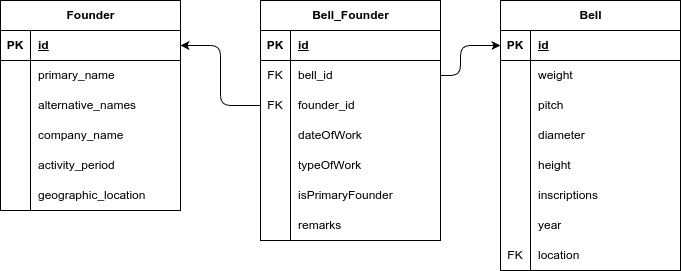
\includegraphics[width=0.3\textwidth]{images/founder_bell.png}
    \caption{Relationship between founder and bell entity.}
    \label{fig:founder_bell-relation}
\end{figure}


\subsection{tower}

The tower entity is the geographical location where the bell is located. It is possible that a bell is not located in a tower, but we still need to document the location of the bell. Then the tower entity can be filled in with minimal attributes and a remark that the bell is not located in a tower. So in this case the tower name is a more generic class in our model, but since most bells are located in a tower, we can use the name for it to make the model more readable.

The items in the tower entity are:

\begin{itemize}
    \item \textbf{Name:} The name of the tower
    \item \textbf{Building:} The building attached to the tower, can be a church or can be empty when the tower in it self has a clear name.
    \item \textbf{Geo Coordinates:} The geographical coordinates of the tower in longitude and latitude.
    \item \textbf{Adress:} The adress of the tower.
    \item \textbf{height:} The height of the tower.
    \item \textbf{height bell:} The approxamte height of the bell in the tower.
    \item \textbf{remark:} A remark about the tower, can be used to document that the bell is not located in a tower or other remarks.
\end{itemize}

\begin{figure}[h!]
    \centering
    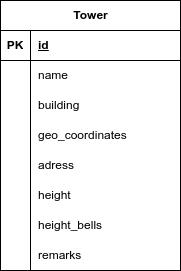
\includegraphics[width=0.3\textwidth]{images/tower.png}
    \caption{Minimal attributes for the tower entity.}
    \label{fig:tower-entity}
\end{figure}

\subsubsection{Relationship Bell - Tower}

The relationship between the \textbf{bell} and its location (\textbf{tower}) represents another \textbf{many-to-many association} with historical significance. Throughout their lifetimes, bells frequently migrate between locations — sometimes due to renovations, institutional changes, or preservation efforts. While documenting a bell's current location unambiguously is essential for practical access and research, capturing its complete spatial history provides valuable context for understanding its cultural and historical significance.

This temporal-spatial complexity necessitates a dedicated relationship table with attributes that document when and why location changes occurred. The relationship entity should contain:

\begin{itemize}
    \item \textbf{Time Period:} Start and end dates of the bell's presence at a location
    \item \textbf{Current Location Flag:} Boolean indicator of the bell's present location
    \item \textbf{Reason for Movement:} Documentation of why the bell was relocated
    \item \textbf{Installation Details:} Information about the bell's mounting, accessibility, and position
\end{itemize}

This approach ensures researchers can quickly identify a bell's current location while preserving its complete geographical provenance for historical analysis and cultural heritage documentation.

\begin{figure}[h!]
    \centering
    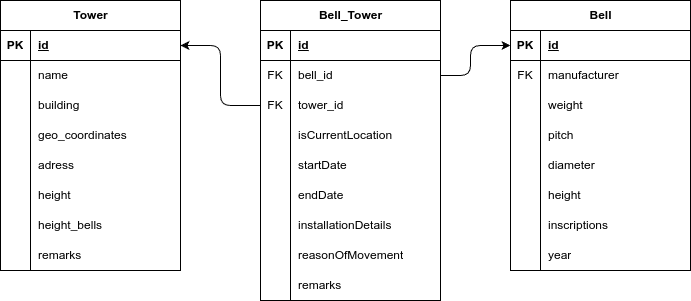
\includegraphics[width=0.3\textwidth]{images/tower_bell.png}
    \caption{Relationship between tower and bell entity.}
    \label{fig:tower_bell-relation}
\end{figure}

\subsection{Carillon}

The carillon entity is used to group bells in to a bigger entity, we know as a carillon. Since we sometimes have infomation on a carillon but less on individual bells,
it should be possible to manually enter some calculated information on the carillon.
This also can be calculated automatically if all bells are all entered in the database. 

The items in the carillon entity are:

\begin{itemize}
    \item \textbf{Tower:} The tower where the carillon is located. (Other entity)
    \item \textbf{Established:} Year that the carillon was installed.
    \item \textbf{Number of bells:} The number of bells in the carillon.
    \item \textbf{Total weight:} The total weight of the carillon.
    \item \textbf{Transposition:} The pitch of the C bell in the carillon.
    \item \textbf{Keyboard Standard:} The keyboard standard used in the carillon.
    \item \textbf{Remark:} A remark about the carillon.
\end{itemize}

\begin{figure}[h!]
    \centering
    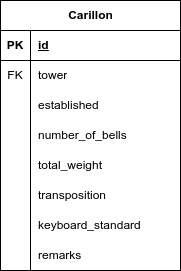
\includegraphics[width=0.3\textwidth]{images/carillon.png}
    \caption{Minimal attributes for the carillon entity.}
    \label{fig:carillon-entity}
\end{figure}

\subsubsection{Relationship Carillon - Bell}

The relationship between carillons and bells represents another \textbf{many-to-many association} with both temporal and conceptual dimensions. A carillon comprises multiple bells, while individual bells may belong to different carillons throughout their history — either through physical relocation or through significant transformations of the carillon itself. 

This latter case presents an interesting ontological challenge: when a carillon undergoes substantial renovation, expansion, or reconfiguration, campanologists may consider it a new instrument despite maintaining some original elements. The determination of whether modifications constitute a new carillon or merely an evolution of the existing one often involves subjective judgment informed by factors such as:

\begin{itemize}
    \item \textbf{Scope of Change:} The percentage of bells replaced or added
    \item \textbf{Keyboard Modification:} Significant alterations to playing mechanisms
    \item \textbf{Tonal Transformation:} Fundamental changes to the instrument's musical character
    \item \textbf{Historical Discontinuity:} Periods of disuse or complete dismantling between configurations
\end{itemize}

Rather than imposing rigid classification rules for these complex cases, our model accommodates the evolving consensus of the campanological community. The relationship table allows documentation of bell membership in multiple carillon configurations while preserving the historical narratives that connect them. Database managers are advised to follow established conventions within the field while documenting the rationale for classification decisions in accompanying notes.

This approach balances the need for structured data with respect for the nuanced historical judgments that characterize campanological scholarship.

\begin{figure}[h!]
    \centering
    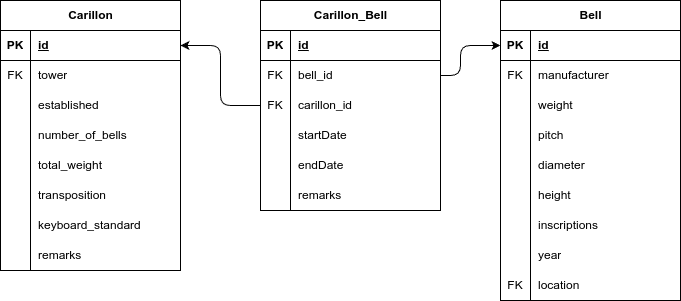
\includegraphics[width=0.3\textwidth]{images/carillon_bell.png}
    \caption{Relationship between carillon and bell entity.}
    \label{fig:carillon_bell-relation}
\end{figure}

\section{Entity Relationship Diagram}

When we put the entities and the relationships between the entities in a diagram, we get a clear overview of the database schema. This diagram can be used as a minimum for the standard in the field of campanology. This schema can be used as a starting point, but is easely extendable with more entities and even relationships. But by maintaining the basis of the database schema, we can ensure that the databases accross the field are compatible and connectible. 

The basic ERD is also extended with a \textbf{File entity}. This entity is used to couple files to other entities in the database, and enrich the data with pictures, audio, articles and more. This entity is not mandatory, but can be used to make the database more usefull and complete.

\clearpage

\begin{figure}[h!]
    \centering
    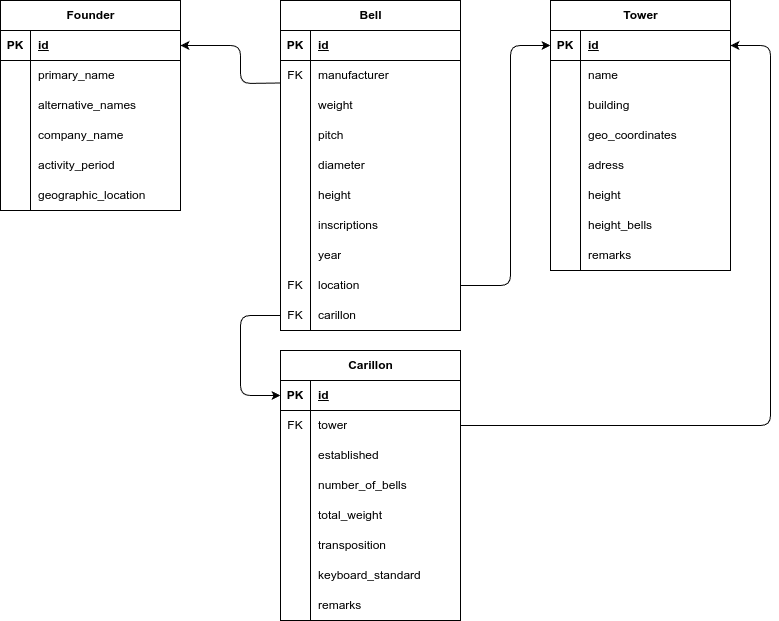
\includegraphics[width=0.8\textwidth]{images/basic_erd.png}
    \caption{Basic ERD for the campanological database schema.}
    \label{fig:basic-erd}
\end{figure}

\section{Conclusion}

This research addresses a gap in the field of campanology by proposing a standardized database schema for comprehensive bell heritage documentation. Our approach is distinguished by several key characteristics that balance standardization with flexibility:

First, by identifying four core entities—bells, founders, towers, and carillons — with their essential attributes and complex interconnections, we establish a minimal but sufficient framework that can serve diverse documentation needs. This framework accommodates the historical complexity inherent to campanological research, particularly the temporal and conceptual challenges posed by evolving relationships between entities over centuries.

Second, our proposed schema recognizes and addresses the unique ontological challenges of campanological documentation, such as the subjective determination of when modifications constitute a new carillon, the complexities of founder attribution across time, and the migratory nature of bells throughout their lifespans. Rather than imposing rigid classification systems, the model incorporates flexibility while maintaining structural integrity.

Third, by designing the schema as an extensible foundation rather than an exhaustive prescription, we enable adaptation to specific research contexts while preserving cross-institutional compatibility. This approach respects the valuable domain expertise of both professional researchers and amateur enthusiasts, allowing specialized documentation within a standardized framework.

Looking forward, the complementary \textbf{open-source Django web application} currently in development will make this schema accessible to organizations with limited technical resources. Future work should focus on developing further standarized measurments and naming conventions to complement the structural standards proposed here. 

In conclusion, this standardized schema represents an important step toward transforming isolated bell documentation efforts into an interconnected network of compatible datasets. While acknowledging that complete standardization across all campanological documentation may remain elusive, this framework offers a practical balance between structure and flexibility that can significantly enhance collaborative research opportunities and comprehensive analysis across the rich and diverse field of campanology.

\section{References}

\bibliographystyle{apalike}
\bibliography{references}

\end{document}